\section{評価}
\pagenumbering{arabic}

\subsection{評価環境}
評価の目的・手法・実験環境

評価環境も図にする

\subsection{クラウドゲームサーバ・クライアント間の通信性能}

\subsubsection{リンクに対する生の遅延の大小の影響}
tcを使って任意に遅延を挿入し、pingの値で遅延の増え方に影響がないか見る。
遅延が増えたときの遅延の増え方が線形みたいなことを言う。
遅延が増えたときの帯域の減り方の話をする。

\subsubsection{リンクに対する遅延の大小の帯域への影響}
tcを使って任意に遅延を挿入し、iperfで帯域の減り方への影響を見る
遅延が増えたときの帯域の減り方の話をする。

\subsection{ゲームプレイ時のフレームレート}

\subsubsection{ネットワーク帯域の大小の影響}
tcを使って帯域に制限をかけて、実際に複数のゲームをプレイしたときのフレームレートへの影響を見る。
使用したゲームはSteamで公開されているAlbion Online(MMORPG)、Red Eclipse 2(FPS, Action)、Simply Chess(Board Game)


\begin{figure*}[t]
    \centering
    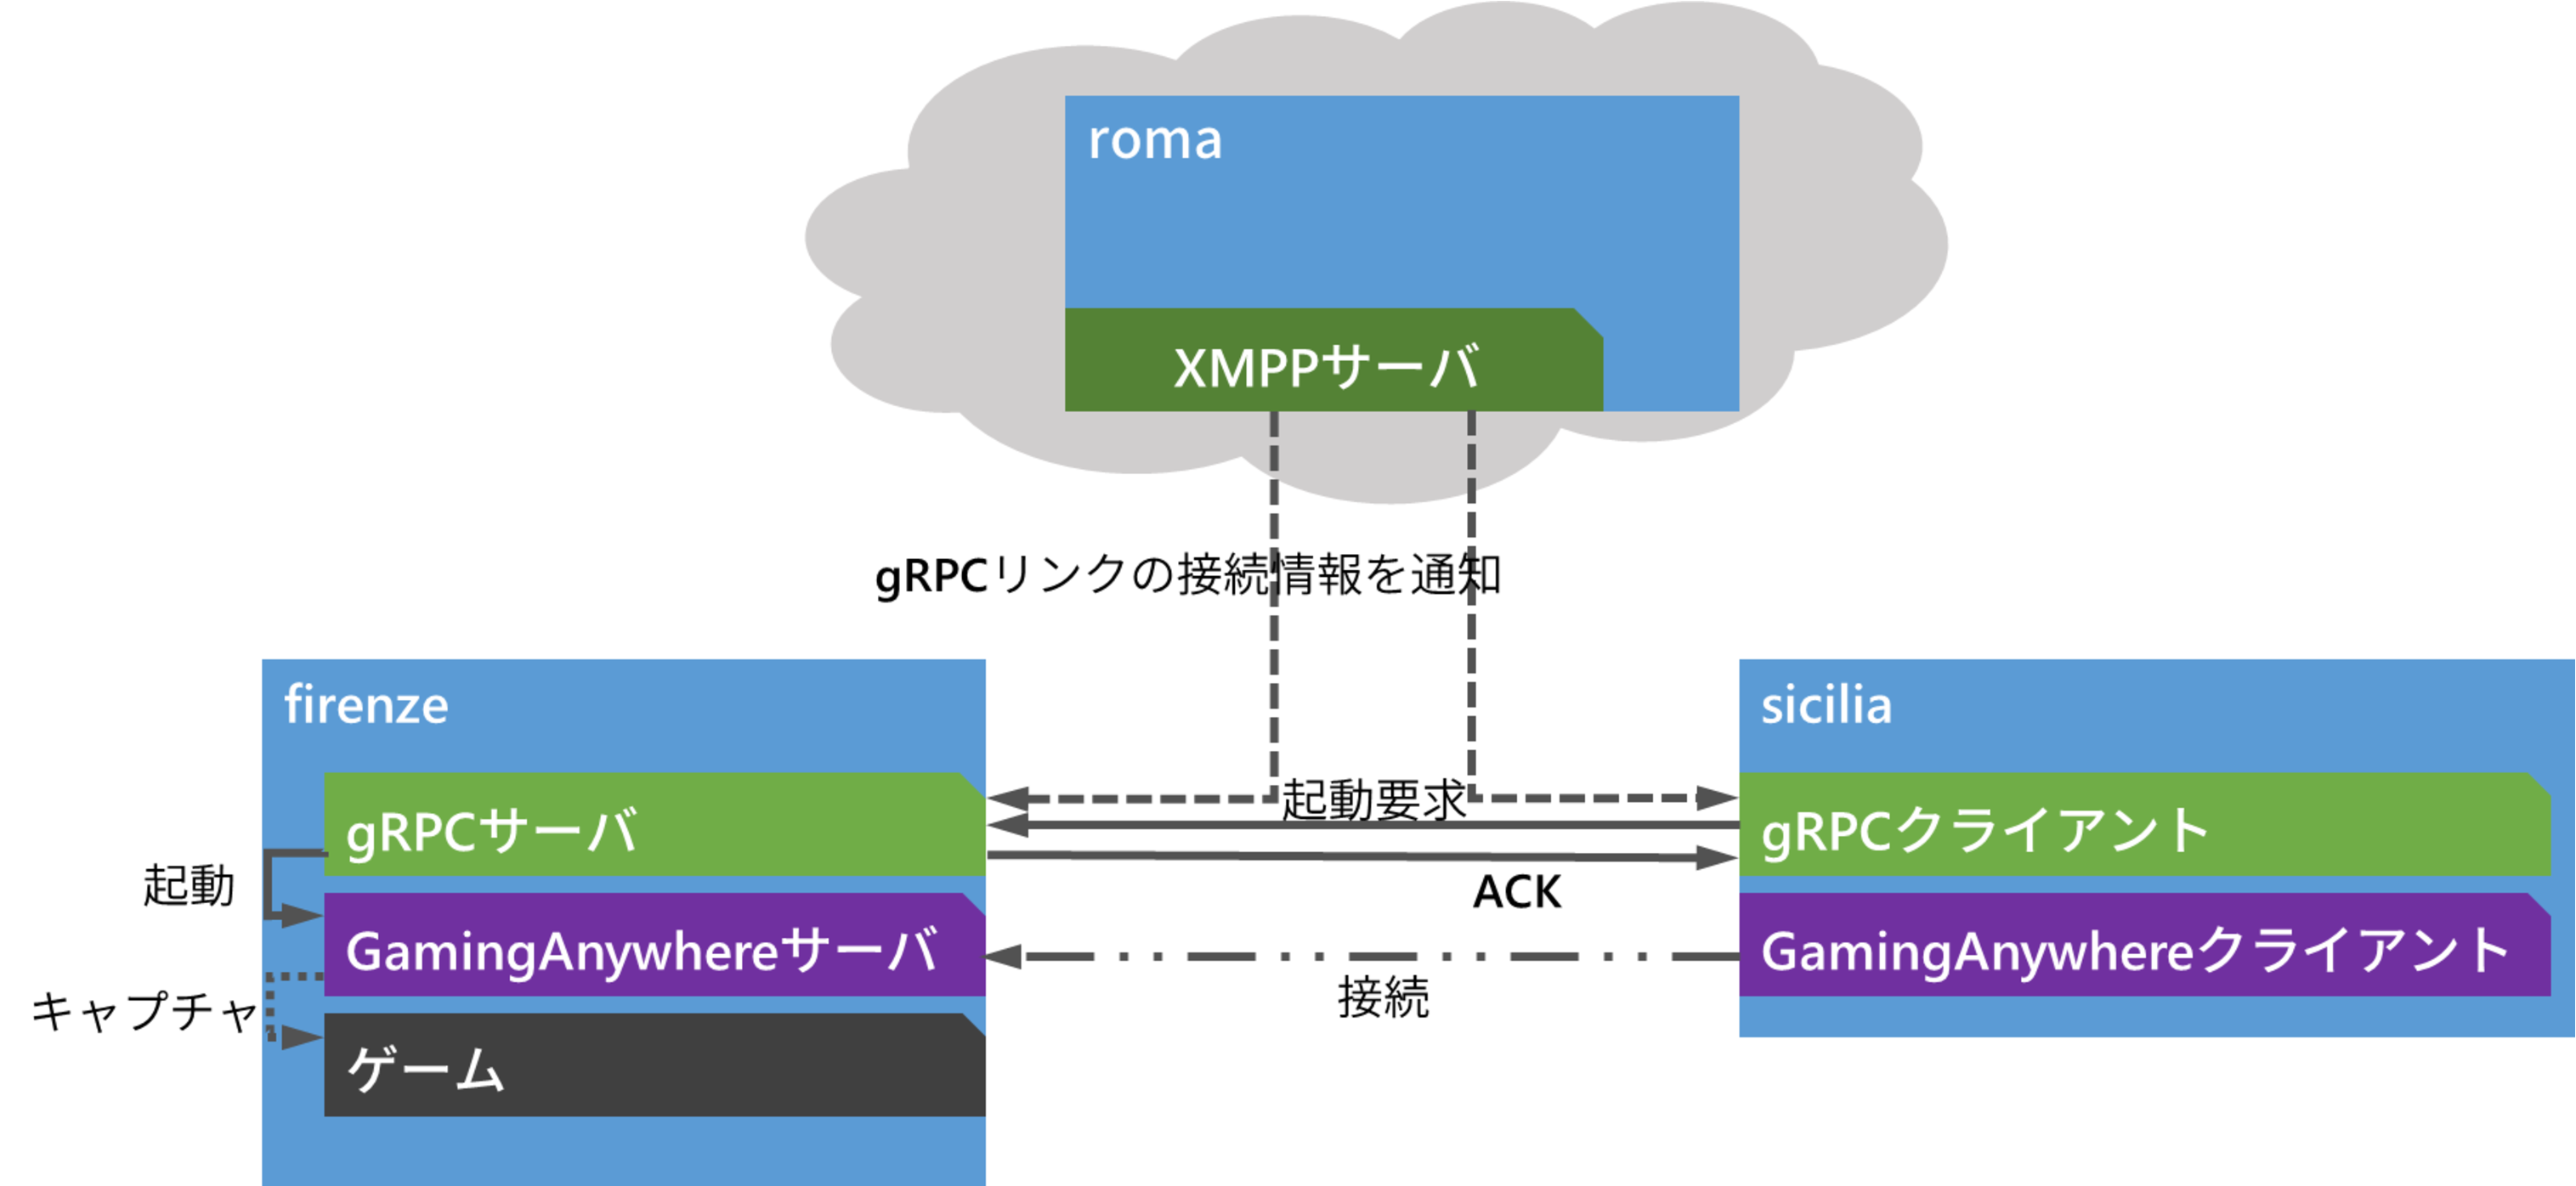
\includegraphics[width=0.8\textwidth,keepaspectratio,clip]{img/experimentalenvironment.pdf}
    \caption{評価環境}
    \label{fig:expenv}
\end{figure*}

\begin{figure*}[t]
    \centering
    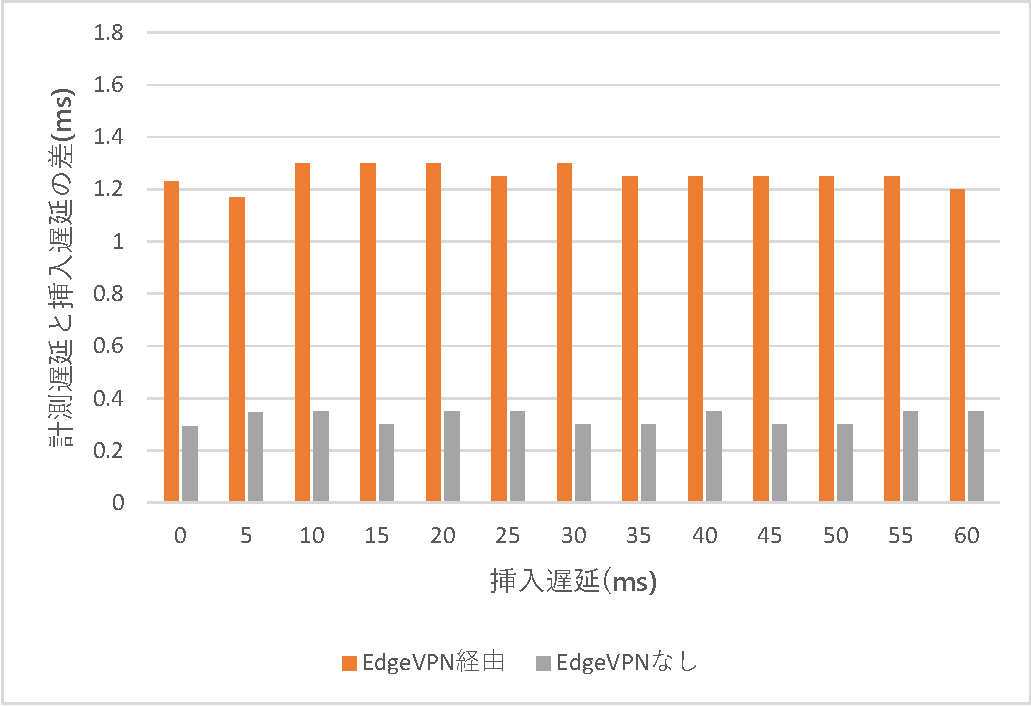
\includegraphics[width=0.8\textwidth,keepaspectratio,clip]{img/graph_ratency.pdf}
    \caption{EdgeVPNリンクに対する遅延挿入の影響}
    \label{fig:ratency}
\end{figure*}

\begin{figure*}[t]
    \centering
    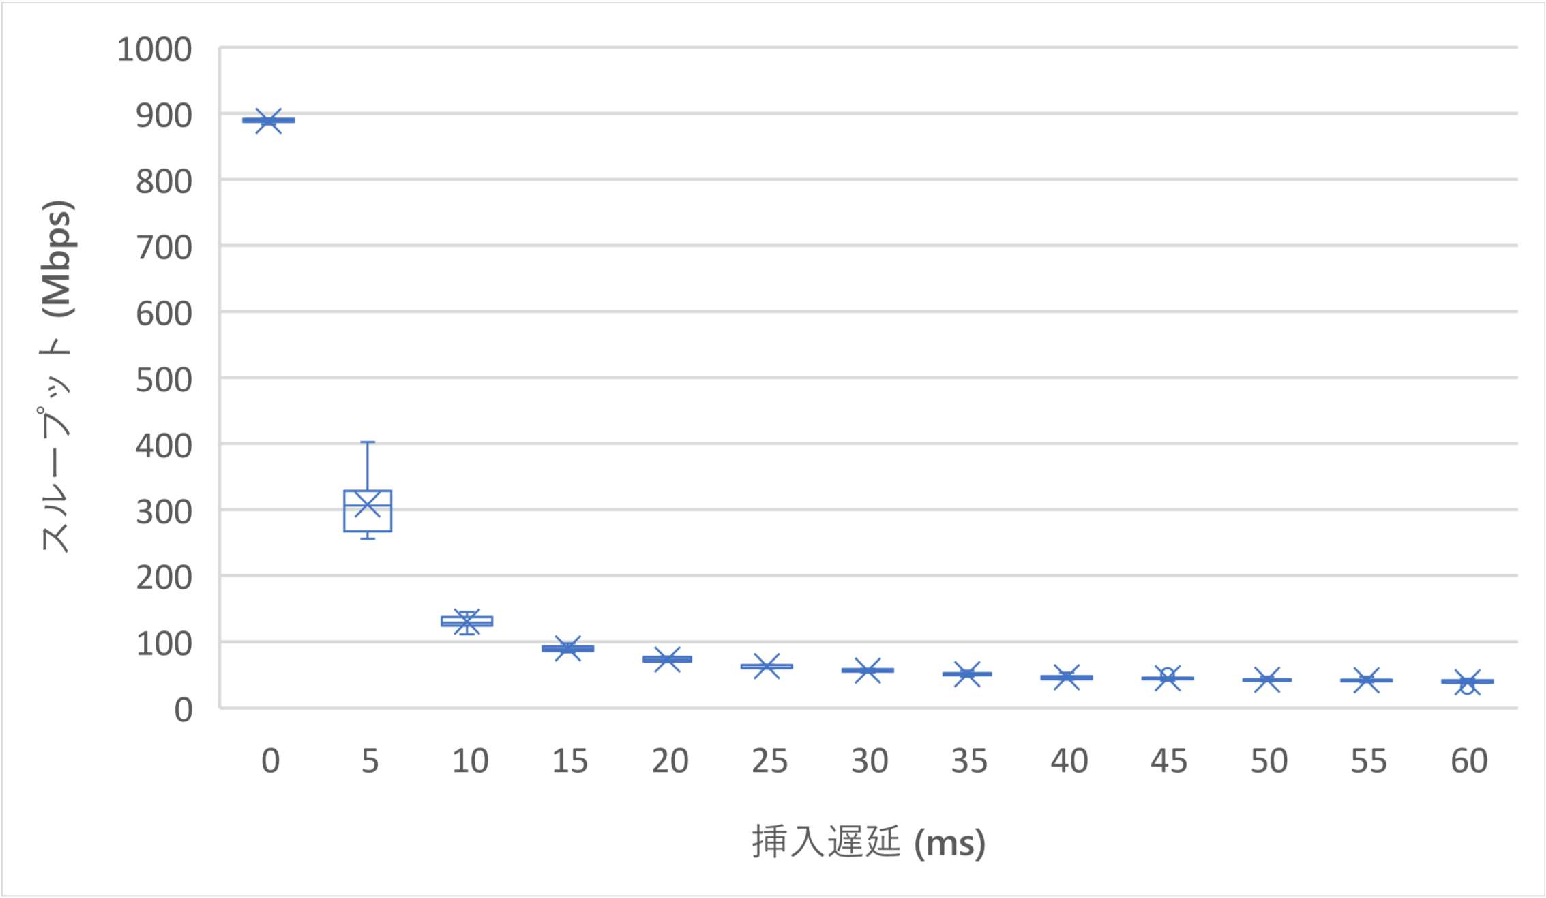
\includegraphics[width=0.8\textwidth,keepaspectratio,clip]{img/bandwidth_withEdgeVPN.pdf}
    \caption{EdgeVPNリンクへの遅延挿入の帯域への影響}
    \label{fig:band_with_edge}
\end{figure*}

\begin{figure*}[t]
    \centering
    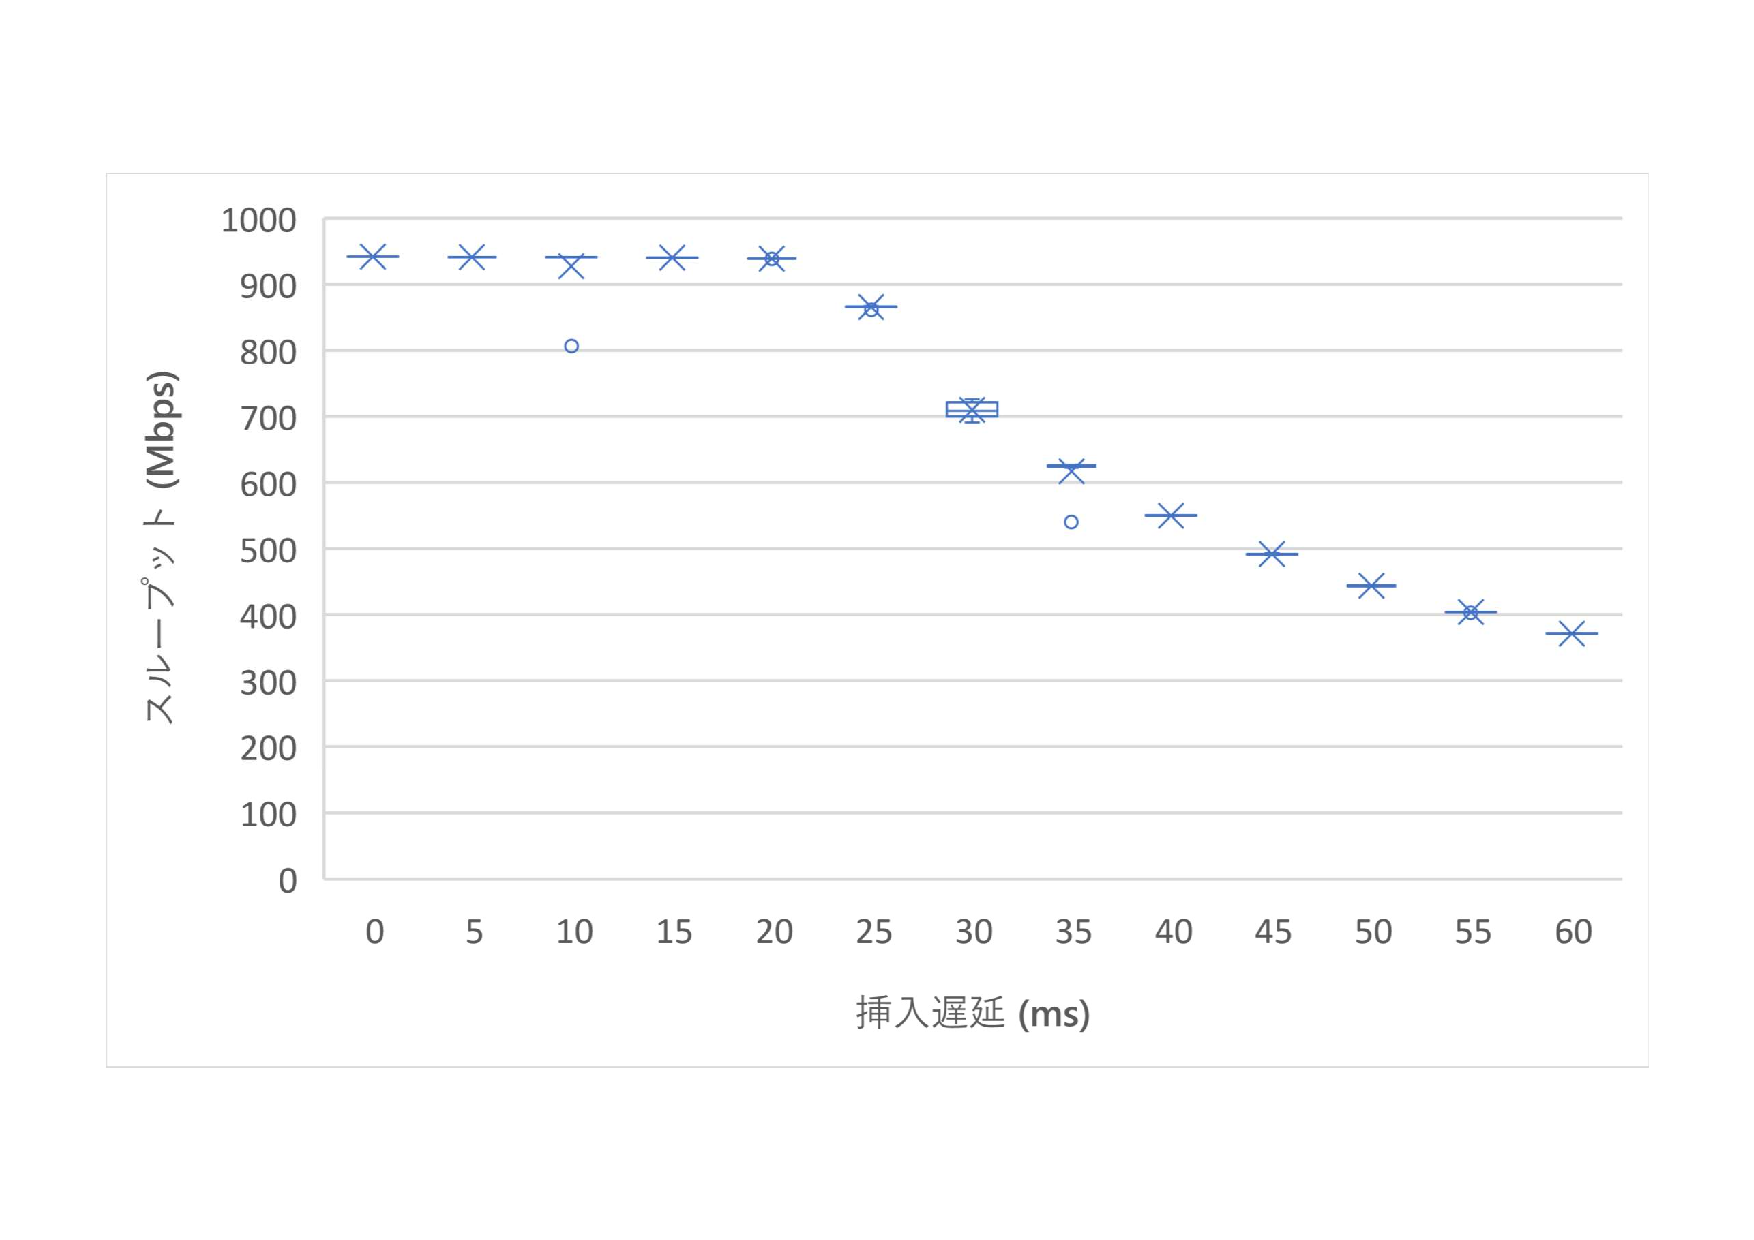
\includegraphics[width=0.8\textwidth,keepaspectratio,clip]{img/bandwidth_withoutEdgeVPN.pdf}
    \caption{EdgeVPNを使用していないリンクへの遅延挿入の帯域への影響}
    \label{fig:band_without_edge}
\end{figure*}

\begin{figure*}[t]
    \centering
    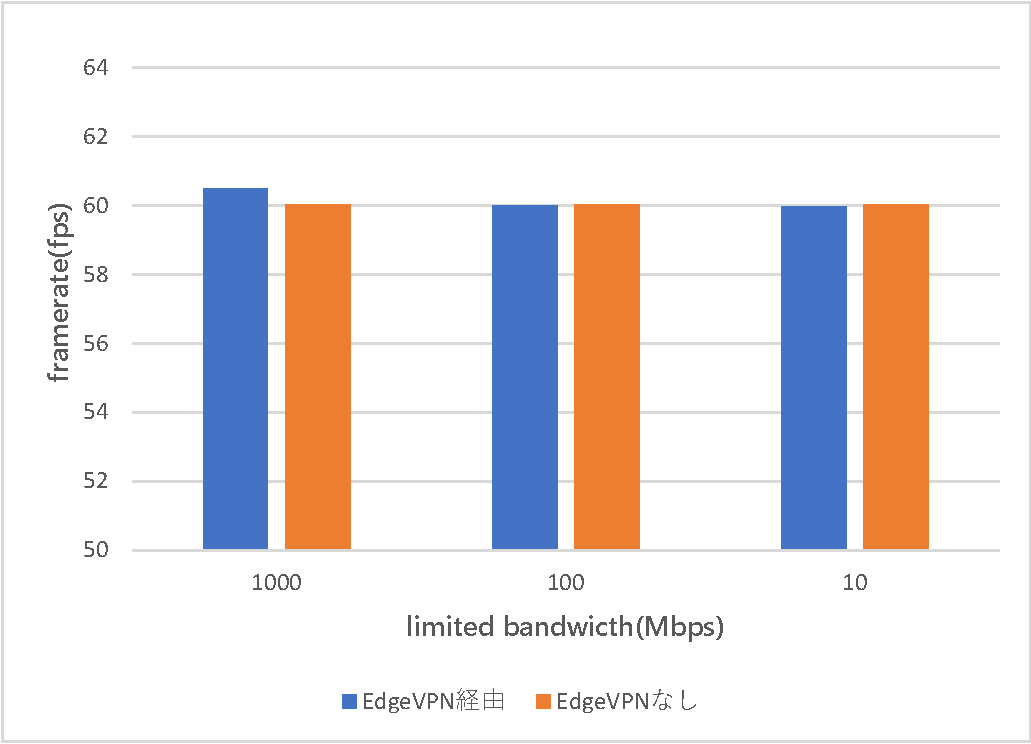
\includegraphics[width=0.8\textwidth,keepaspectratio,clip]{img/framerate_MMO.pdf}
    \caption{帯域制限下でのゲームプレイ時のフレームレートの変化 (Albion Online (MMORPG)プレイ時)}
    \label{fig:fps_mmo}
\end{figure*}

\begin{figure*}[t]
    \centering
    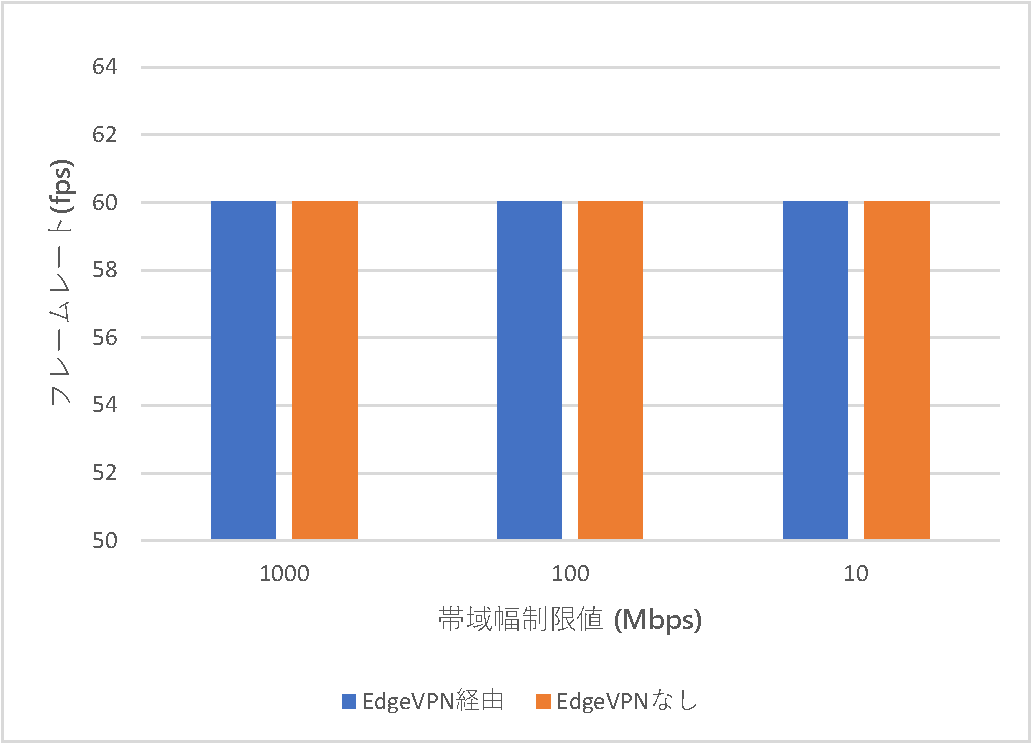
\includegraphics[width=0.8\textwidth,keepaspectratio,clip]{img/framerate_FPS.pdf}
    \caption{帯域制限下でのゲームプレイ時のフレームレートの変化 (Red Ecliplse 2 (FPS, Action)プレイ時)}
    \label{fig:fps_fps}
\end{figure*}

\begin{figure*}[t]
    \centering
    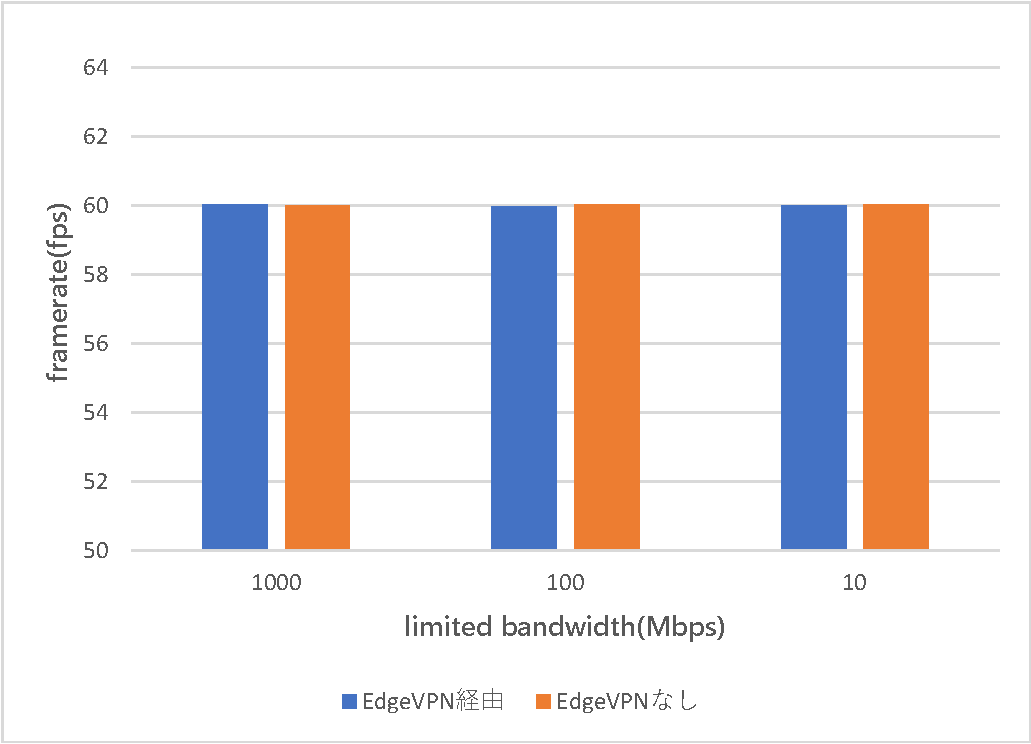
\includegraphics[width=0.8\textwidth,keepaspectratio,clip]{img/framerate_Board.pdf}
    \caption{帯域制限下でのゲームプレイ時のフレームレートの変化 (Simply Chess (ボードゲーム)プレイ時)}
    \label{fig:fps_board}
\end{figure*}